\documentclass[norsk, 10pt]{article}
\usepackage{babel}          % Ordelingsregler, osv
\usepackage[utf8]{inputenc}
\usepackage[T1]{fontenc}
\usepackage{booktabs}       % Ordentlige tabeller
\usepackage{url}            % Skrive url-er
\usepackage{textcomp}       % Den greske bokstaven micro i text-mode
\usepackage{units}          % Skrive enheter riktig
\usepackage{float}          % Figurer dukker opp der du ber om
\usepackage{lipsum}         % Blindtekst
\usepackage{amsmath, amsfonts, amssymb, amsthm}
\usepackage{caption,subfigure,listings, booktabs}
\usepackage{tikz,graphicx}
\usepackage{sectsty}

% Setter fonter
\usepackage{bbold,gillius}
\allsectionsfont{\sffamily} % Sans serif på alle overskrifter
%\renewcommand{\abstractname}{Executive Summary}
\captionsetup{width=.9\textwidth, textfont={small,it},labelfont={small,sf}}
\usepackage[sc,osf]{mathpazo} % Palatino


% Kodelisting
\usepackage{verbatim}
\lstset{language=matlab,breaklines=true,numbers=left} % For hele programmer.
%\lstinputlisting[language=matlab]{fil.m}

% Layout
\usepackage[top=1.2in, bottom=1.7in, left=1.7in, right=1.7in]{geometry}
%\usepackage[top=1.2in, bottom=1.7in, left=.7in, right=.7in]{geometry}
\frenchspacing % Rett mellomrom etter punktum.
\linespread{1.1} % Linjeavstand.
\usepackage[colorlinks=true]{hyperref} % Farge på lenker.

% Egendefinerte kommandoer
\newcommand{\dt}{\, {\rm d}t\, }
\newcommand{\dx}{\, {\rm d}x\, }
\newcommand{\dv}{\, {\rm d}v\, }
\newcommand{\dr}{\, {\rm d}r\, }
\newcommand{\dd}{\, {\text d} }
%\newcommand{\dp}{\ {\rm d}p\ }
\newcommand{\R}{\mathbb{R}}
\def\mean#1{\left\langle #1 \right\rangle}
\renewcommand{\exp}{\mathit{e}}
%\DeclareMathOperator{\dt}{dt}
\newcommand{\mb}[1]{\mathbf{#1}}
\def\para#1{\left( #1 \right)}
\newcommand{\ket}[1]{\left|#1\right\rangle}
\newcommand{\bra}[1]{\left\langle#1\right|}

%, trim = 1cm 7cm 1cm 7cm % PDF-filer som bilde

\begin{document}

% Forside
\begin{titlepage}
\begin{center}

\textsf{\Large FYS4150 - Computational Physics\\[0.5cm]
\rule{\linewidth}{0.5mm} \\[0.4cm]
{ \huge \bfseries  PROSJEKT 4}\\[0.10cm]
\rule{\linewidth}{0.5mm} \\[1.5cm]
{\Large Isingmodellen, Monte Carlo og parallellisering}}\\[1.5cm]
\textsc{}\\[1.5cm]

% Av hvem?

\textsf{\begin{minipage}{0.49\textwidth}
    \begin{center} \large
        Kandidat 72
    \end{center}
\end{minipage}}
%\begin{minipage}{0.49\textwidth}
%    \begin{center} \large
%        Anne-Marthe Hovda\\ \url{annemmho@uio.no} \\[0.8cm]
%    \end{center}
%\end{minipage}}


\vfill

% Dato nederst
\textsf{\large{Dato: \today}}

\end{center}
\end{titlepage}

\abstract{}


\section*{Introduksjon}
% Hva er Isingmodellen
I dette prosjektet skal vi se på den todimensjonale Isingmodellen ved hjelp av numeriske beregninger. Isingmodellen er en statistisk(???) modell for et ferromagnetisk system der vi har diskrete variabler organisert i et gitter, de diskrete variablene vil i vårt tilfelle kunne ta verdiene $1$ og $-1$, henholdsvis spinn opp og spinn ned. Hvert spinn i gitteret vekselvirke med de fire næreste naboene.

% Metropolisalgoritmen
For å simulere dette systemet på en datamaskin må vi bruke en egnet algoritme, i vårt tilfelle benytter vi Metropolisalgoritmen. Den er en ganske enkel, men kraftig algoritme. Kort sagt går den ut på å sammenlikne en prøvetilstand av systemet med en starttilstand og så akspetere eller avvise den nye tilstanden ved å bruke en akseptering- og avvisningsrutine.

% MC
Når vi bruker Metropolisalgoritmen så har vi behov for genererte tilfeldige tall, det kan vi få ved å bruke Monte Carlo-metoder. Vi har laget et program som løkker over alle matriseelementer for hver Monte Carlo-syklus, og for hvert matriseelement som blir løkket over så velger vi et tilfeldig element i matrisa som får spinnet sitt snudd. 

% Hva er parallellisering og litt om faseovergang
Til slutt i prosjektet så parallelliserer vi koden slik at vi kan kjøre den for flere temperaturer på en forholdsvis rask måte. Parallelliseringa er gjort på en måte slik at vi beregner for så mange temperaturer som det er kjerner å kjøre på i maskinen vi bruker. Når vi kjører en slik beregning så kan vi plotte de forskjellige verdiene som beskriver systemet, som en funksjon av temperatur. Vi vil da kunne finne hvor eventuelle faseoverganger skjer.

\section*{Teori}
% Isingmodellen
Vi kan bruke termofysikk til å finne egenskapene til systemet vårt, vi er først og fremst interessert i å finne partisjonsfunksjonen siden vi kan finne snittenergi, varmekapasitet, snittmagnetisering, og susceptibilitet når vi kjenner den. Partisjonsfunksjonen er
$$ Z = \sum\limits_{i=1}^{M} e^{-\beta E_i}, $$
hvor $\beta = 1/k_B T$, der $k_B$ er Boltzmanns konstant som setter lik $1$, og vi summerer over alle mikrotilstander i systemet. Energien er enkel å finne, det er bare å telle opp alle vekselvirkningene spinnene har med hverandre og et eventuelt bidrag fra vekselvirkningene mellom et eksternt magnetfelt $B$ og spinnene i systemet vårt. I vårt tilfelle er det ikke noe eksternt magnetfelt, så vi får,
$$ E_i = -J\sum\limits_{\mean{j,k}}^{L} s_js_k, $$
hvor $\mean{j,k}$ betyr at vi summerer over de næreste naboene. Siden gitteret vårt er endelig, så må vi bestemme oss for hvordan vi skal behandle endene. Vi er interessert i å ha en modell som simulerer virkeligheten best mulig, så vi velger å ha periodiske randbetingelser. Det betyr at vi kobler sammen endene på vårt to-dimensjonale gitter slik at vi effektivt får en torus.

For enkelhetsskyld så ser vi på et én-dimensjonalt system for å finne ut hvordan vi skal summere sammen energiene. Vi kan ha f.eks. tre spinn som peker opp,
$$ \uparrow_1\quad\uparrow_2\quad\uparrow_3\quad, $$
hvor vi da har tre vekselvirkninger, $\uparrow_1\uparrow_2$, $\uparrow_2\uparrow_3$ og $\uparrow_1\uparrow_3$. Vi kan skrive dette enkelt som,
$$ E_i = -J\sum\limits_{j}^{L} s_js_{j+1}, $$
hvor $s_1 = s_{N+1}$, altå vår randbetingelse. Når vi så skal gjøre dette i to dimensjoner så kan vi tenke oss at den ene summen går radvis i gitteret, mens den andre går kolonnevis, slik at vi får to dobbeltsummer,
\begin{align*}
	E_i &= -J\sum\limits_{j}^{L}\sum\limits_{n}^{L} s_{n,j}s_{n,j+1} - J\sum\limits_{j}^{L}\sum\limits_{n}^{L} s_{n,j}s_{n+1,j}\\
	&= -J\sum\limits_{j}^{L}\sum\limits_{n}^{L} s_{n,j}(s_{n,j+1} + s_{n+1,j}).
\end{align*}
der vi har implementert randbetingelsene på samme måte som over. Vi kan nå enkelt finne partisjonsfunksjonen, i det minste for systemer med $L=2$. Det blir fort mange mikrotilstander å telle over når $L$ øker, men heldigvis for oss klarte Onsager å finne en analytisk løsning for partisjonsfunksjonen når $L\to\infty$, slik at vi kan sammenlikne vår numeriske løsning og hvordan den vil utvikle seg når vi øker $L$ i beregningene våre.

Vi kan nå finne partisjonsfunksjonen for $L=2$ og deretter \emph{enhets}teste programmet vårt for å se om det gir riktig resultat. For $L=2$ har vi $2^{4}=16$ mikrotilstander. De kan vi enkelt tegne opp,
\begin{eqnarray}
	\begin{matrix} \uparrow\uparrow \\ \uparrow\uparrow \end{matrix} & \begin{matrix} \downarrow\downarrow \\ \downarrow\downarrow \end{matrix} & 4\cdot \begin{matrix} \uparrow\downarrow \\ \downarrow\downarrow \end{matrix}\\ 2\cdot\begin{matrix} \uparrow\downarrow \\ \downarrow\uparrow \end{matrix} & 4\cdot \begin{matrix} \downarrow\uparrow \\ \uparrow\uparrow \end{matrix} & 2\cdot\begin{matrix} \uparrow\uparrow \\ \downarrow\downarrow \end{matrix}.
\end{eqnarray}
Vi har ganget med degenerasjonsfaktoren for å vise hvor mange eksemplarer det er av samme mikrotilstand, vi ser at to mikrotilstander er like når naboene er til de samme spinnene i hver tilstand er like. Vi finner så energiene ved å bruke summasjonsformelen vi kom fram til i stad, vi ser at systemet enten har energi $E = 8J$ (mikrotilstanden med to spinn opp og like nabospinn for) eller $E = -8J$ (alle spinn opp eller ned), partisjonsfunksjonen blir da,
$$ Z = 2e^{-8\beta J} + 2e^{8\beta J} + 12e^{-\beta \cdot0} = 4\cosh(8\beta J) + 12. $$
Det er nå enkelt å finne uttrykkene for snittenergi og varmekapasitet, de er definert som
\begin{align*}
	\mean E &= -\frac{\partial \ln Z}{\partial \beta} \\
	C_V &= \frac{1}{k_B T^2} \frac{\partial^2}{\partial \beta^2}\ln Z.
\end{align*}
Snittmagnetiseringa er simpelthen summen av alle spinnene delt på antall spinn,
$$ \mean M = \sum\limits_{i=1}^{L} m_i,$$
mens susceptibiliteten er variansen til magnetiseringa,
$$ \chi = \frac{1}{k_BT}(\langle M^2\rangle - \mean M^2).$$
Det er nå ganske rett frem å regne ut de fire størrelsene vi er interessert i.
\begin{align*}
	\mean E &= -\frac{\partial}{\partial \beta} (4\cosh(8\beta J) + 12) \\
	&= -\frac{8J\sinh(8\beta J)}{\cosh(8\beta J) + 3}.
\end{align*}
\begin{align*}
	C_V &= \frac{1}{k_BT^2}\frac{\partial^2}{\partial \beta^2} (4\cosh(8\beta J) + 12) \\
	&= \frac{1}{k_BT^2}\frac{\partial}{\partial \beta} (-\mean E) \\
	&= \frac{1}{k_BT^2}\frac{\partial}{\partial \beta}\frac{8J\sinh(8\beta J)}{\cosh(8\beta J) + 3} \\
	&= \frac{1}{k_BT^2}\para{\frac{64J^2\cosh(8\beta J)}{\cosh(8\beta J) + 3} - \frac{64J^2\sinh(8\beta J)^2}{(\cosh(8\beta J) + 3)^2}} \\
	&= \frac{64J^2}{k_BT^2}\para{\frac{\cosh(8\beta J)}{\cosh(8\beta J) + 3} - \frac{\sinh(8\beta J)^2}{(\cosh(8\beta J) + 3)^2}}
\end{align*}

% HUSK SUSCEPTIBILITET OG GJENNOMSNITTLIG MAGNETISERING

Vi kan velge oss en temperatur og finne de analytiske verdiene, for deretter å kjøre en simulering med Metropolisalgoritmen slik at vi kan sammenlikne resultatene vi får. Dette blir da enhetstesten av programmet vi lager. Nå kan vi se litt nærmere på Metropolisalgoritmen, her så vil vi implementere algoritmen på følgende måte:
\begin{itemize}
\item[1:] Generer en starttilstand
\item[2:] Generer en prøvetilstand, her: snu ett spinn.
\item[3:] Sjekk om prøvetilstanden mot en aksepteringsrutine, her: får systemet en lavere energi aksepterer vi den nye tilstanden ....
\item[4:] Regn ut $w=e^{\beta\Delta E}$ og sammenlikne denne verdien med et tilfeldig tall $r$, hvis $r\leq w$, aksepterer vi den nye tilstanden, hvis ikke så beholder vi den gamle.
\item[5:] Finn de nye forventningsverdiene.
\item[6:] Repeter trinn 2-5 til en god nok tilnærming er oppnådd.
\end{itemize}
For å sjekke når vi har fått en likevektstilstand, så plotter vi hvordan verdiene vi er interesser i, utvikler seg som funksjon av antall MC-sykluser. Vi vil da få en graf som vil flate ut når vi har nådd likevekt. Dette er en ganske ad-hoc måte å sjekke om systemet er i likevekt på, men den er betraktelig enklere enn å regne ut korrelasjonsfunksjoner for å finne når systemet er helt ukorrelert.

Systemet vårt består av $L\times L$ spinn.

% Partisjonsfunksjonen for 2x2-gitter
% ...og tilhørende forventningsverdier for T = 1


\section*{Metode}
Programmet vi har skrevet benytter som allerede nevnt Metropolisalgoritmen for å finne variansen i energi (varmekapasiteten $C_V$), gjennomsnittlig energi $\mean E$, gjennomsnittlig magnetisering $\mean |M|$ og variansen av magnetiseringa (susceptibilitet $\chi$). Før vi kan se ordentlig på disse verdiene så må vi lage et program som vi vet at virker. Vi ser derfor på $2\times2$-tilfellet av et gitter med spinn som kan peke opp eller ned. I forrige seksjon fant vi de analytiske svarene på verdiene vi er interessert i, så vi kan nå enkelt finne ut hvor mange Monte Carlo-sykluser som er nødvendig før vi når et svar som er nøyaktig nok for oss.

Programmet er bygget opp slik at vi kjører for veldig mange MC-sykluser og plotter deretter resultatene som funksjon av antall sykluser. Når vi har et gitter med kun fire spinn så går utregningene ganske raskt, så det er ikke noe problem å ha et høyt antall sykluser. Etter at vi har funnet ut hvor mange sykluser som er nødvendig for å nå likevekt, så kan vi øke størrelsen på gitteret og begynne å samle data etter at vi har nådd likevekt.

Vi vil også se på hvor raskt systemet konvergerer mot likevekt fra en starttilstand der alle spinn peker opp kontra en tilfeldig starttilstand, dette gjør vi for temperaturene $T=1$ og $T=2.4$. Vi vil da plotte gjennomsnittlig energi og magnetisering samt hvor mange aksepterte tilstander som funksjoner av MC-sykluser.

Når vi kjører programmet vårt for flere temperaturer så kjører vi for så mange MC-sykluser at termaliseringa av systemet ikke bidrar nevneverdig til det endelige resultatet vårt. Støyen fra termaliseringa blir ytterligere redusert ved at vi gjenbruker tilstandene. Når vi går ett temperatursteg opp så vil termaliseringa ta kortere tid, det betyr at beregninga for den første temperaturen i hver tråd vil være litt mer unøyaktig enn de påfølgende.


\section*{Resultat}
Vi ser først på resultatene fra enhetstestinga av programmet. Vi simulerte et gitter med $2\times2$ spinn for temperaturene $T=1$ og $T=2.4$, begge med ordnet og uordnet starttilstander. I figurene (\ref{fig:meanET1}), (\ref{fig:varmekapT1}), og (\ref{fig:chiT1}) ser vi resultatene av kjøringer med 10 millioner MC-sykluser for $T=1$. Vi ser at verdiene konvergerer raskt mot en likvektstilstand og at det ikke er nødvendig med 10 millioner MC-sykluser. Standardavvikene er ganske små, så vi kan tillate oss å gå helt ned til én million MC-sykluser når vi skal kjøre for flere temperaturer etter hverandre, som nevnt tidligere vil de påfølgende temperaturstegene ha en kort termaliseringsprosess siden vi kommer til å sette temperatursteget til $\Delta T = 0.01$.

\begin{figure}[H]
\centering
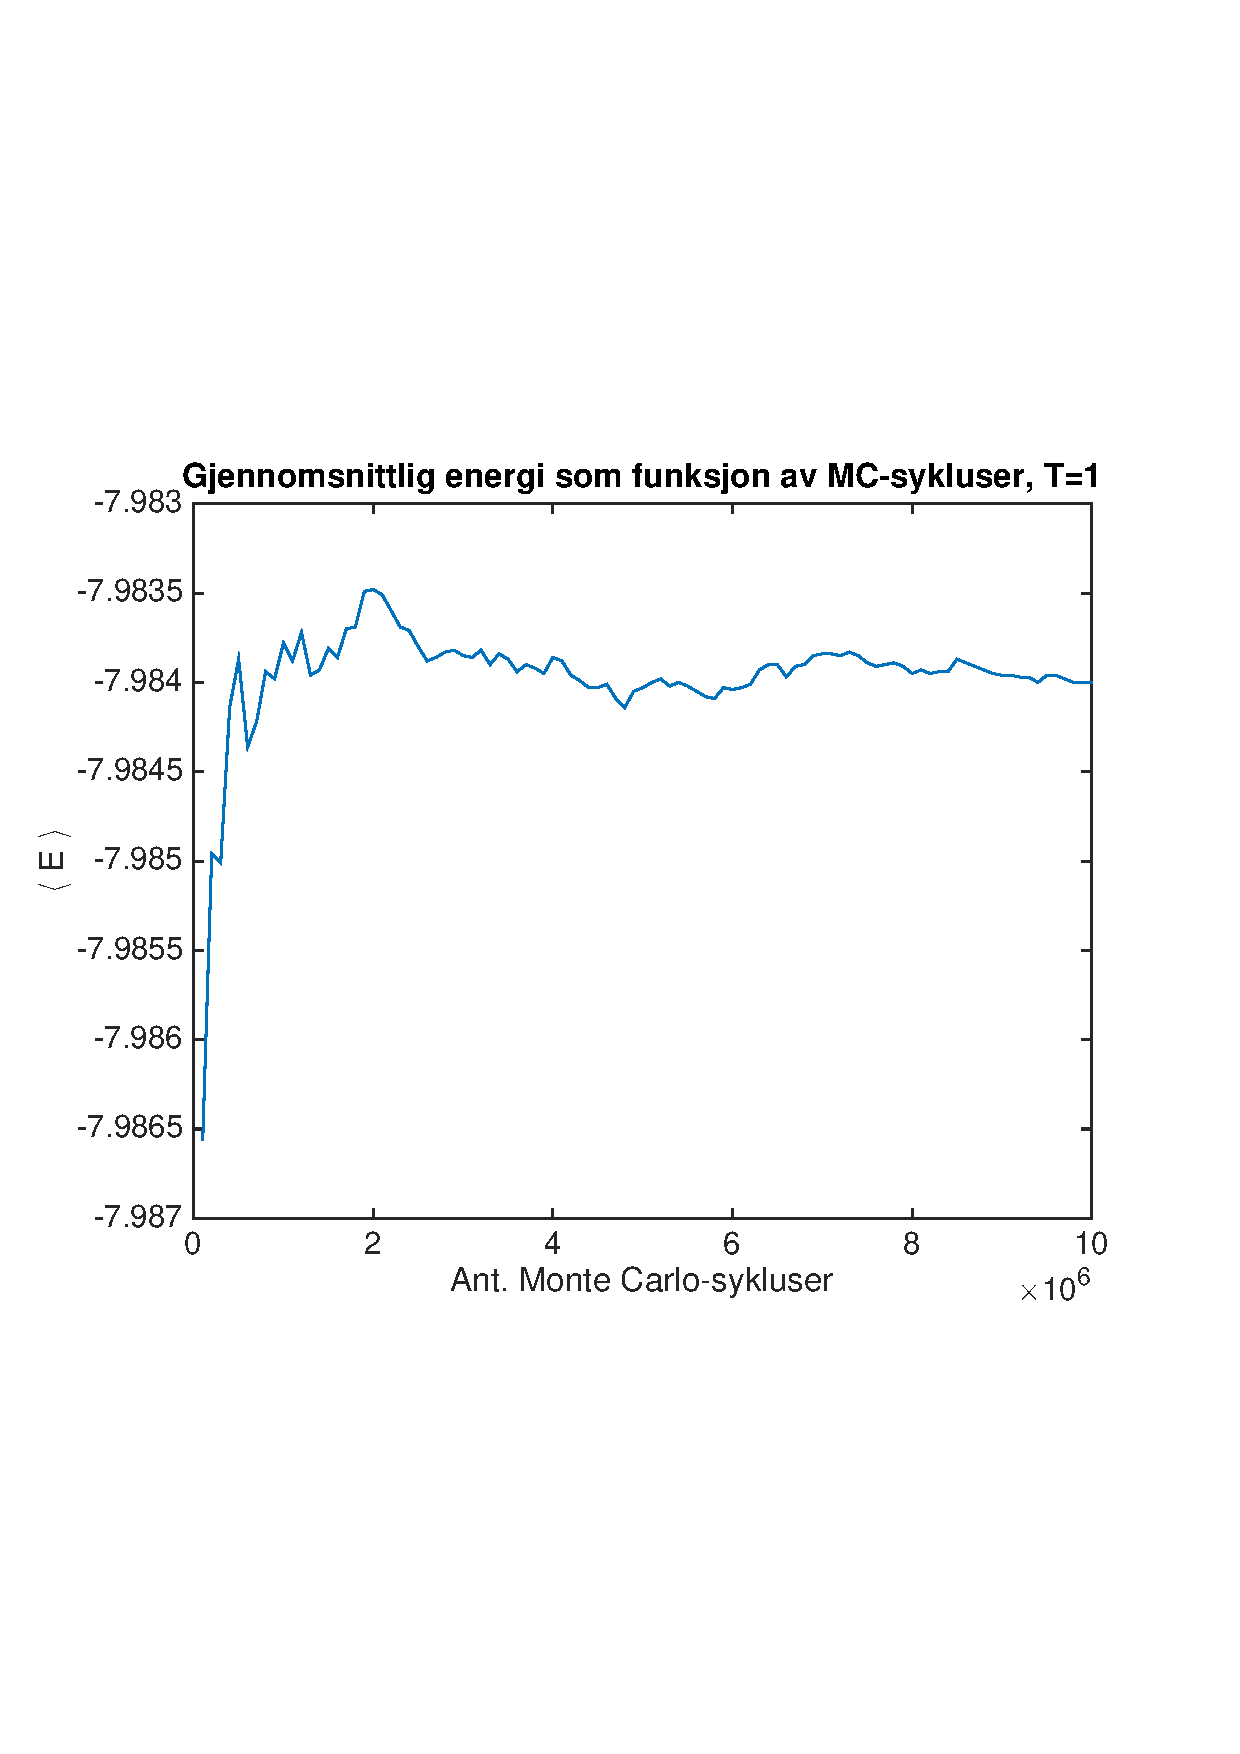
\includegraphics[scale = 0.6, trim = 1cm 8cm 1cm 8cm]{b_avgEnergy_MC_L2_T1.pdf}
\caption{Her er $\mean E$ plottet som funksjon av antall MC-sykluser for ordnet og uordnet starttilstand. Vi ser at første verdi for snittenergien er ganske bra, den treffer på andre desimal, og tar seg raskt inn til likevektstilstanden. Standardavviket til $\mean E$ er $\sigma_{\mean E} = 3.2986\cdot10^{-4}$, som er ganske bra, vi kan da se bort fra termaliseringsprosessen når vi kjører med $4\cdot10^6$ MC-sykluser.}
\label{fig:meanET1}
\end{figure}

\begin{figure}[H]
\centering
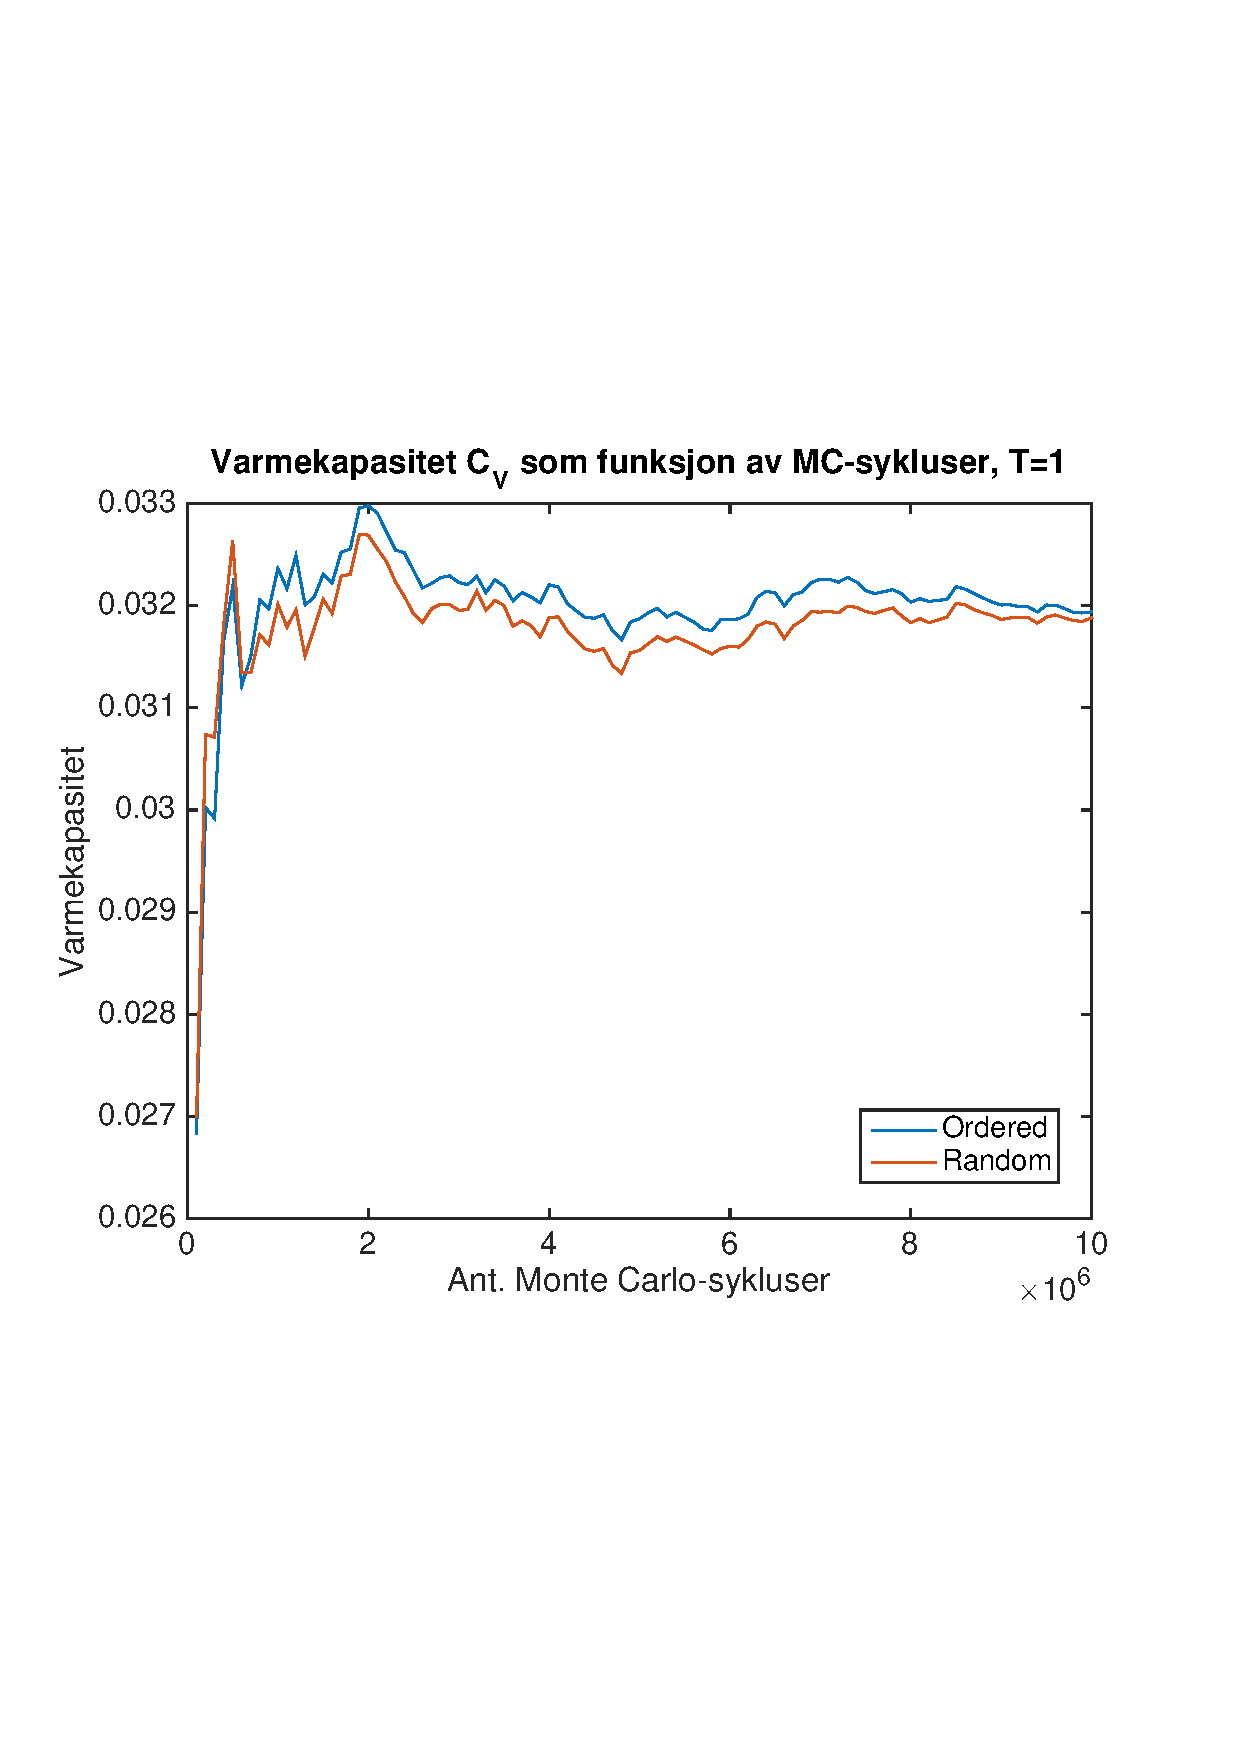
\includegraphics[scale = 0.6, trim = 1cm 8cm 1cm 8cm]{b_varmekap_MC_L2_T1.pdf}
\caption{Vi ser at varmekapasiteten blir estimert litt dårligere i starten enn snittenergien ble, men standardavviket er $\sigma_{C_V} = 6.5732\cdot10^{-4}$. Vi kan altså se bort fra termaliseringa her også.}
\label{fig:varmekapT1}
\end{figure}

\begin{figure}[H]
\centering
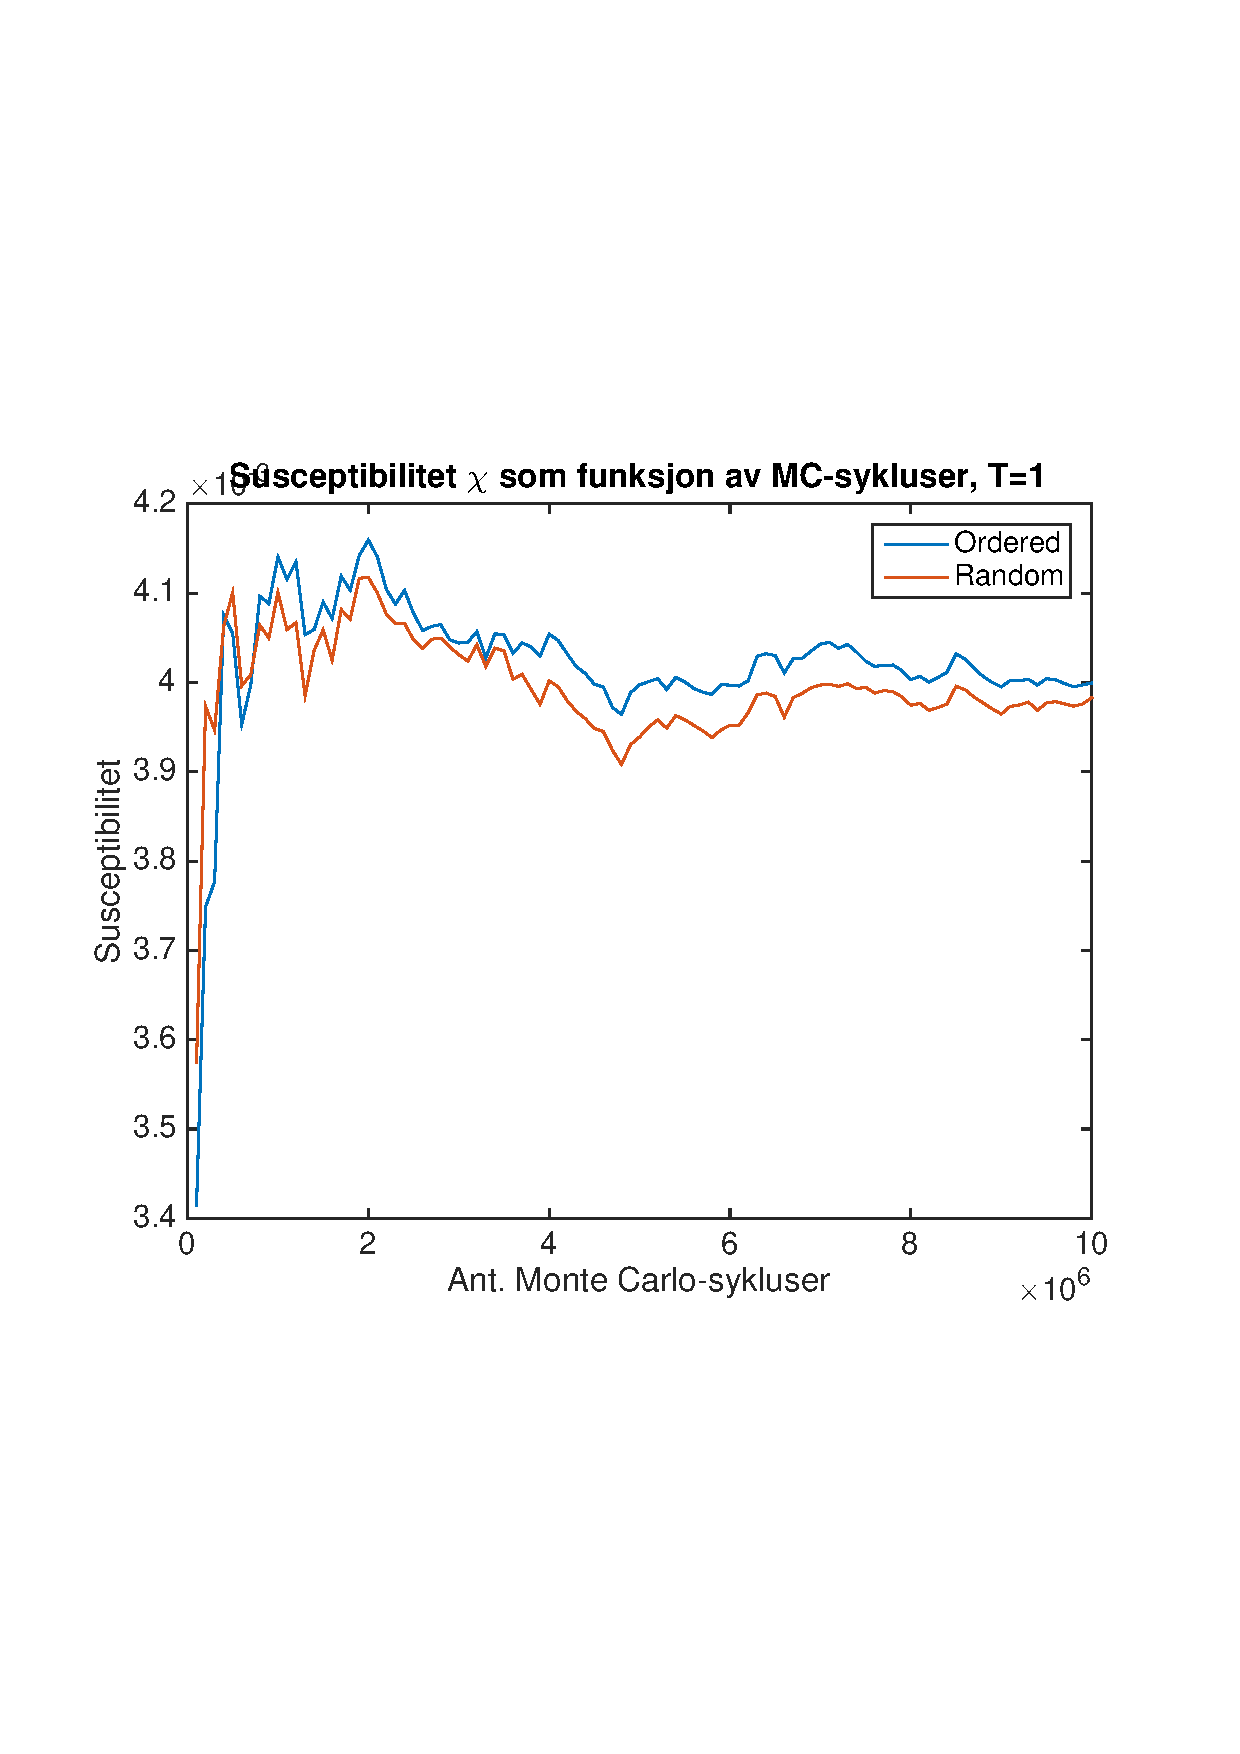
\includegraphics[scale = 0.6, trim = 1cm 8cm 1cm 8cm]{b_chi_MC_L2_T1.pdf}
\caption{Susceptibiliteten får et estimat som er et stykke unna likevektsverdien, men etter to millioner MC-sykluser er den så å si i likevekt. Standardavikket her er $\sigma_\chi = 8.3561\cdot10^{-5}$, som er det laveste av de tre verdiene vi har målt så langt.}
\label{fig:chiT1}
\end{figure}

Vi kan så øke temperaturen til $T=2.4$ og se hvordan forskjellene mellom ordnet uordnet starttilstand er da. I figurene (\ref{fig:meanET24}), (\ref{fig:varmekapT24}), og (\ref{fig:chiT24}) ser vi resultatene. Vi ser at grafene ligger helt oppå hverandre, i noe de ikke gjorde for $T=1$. Dette skjer fordi 

\begin{figure}[H]
\centering
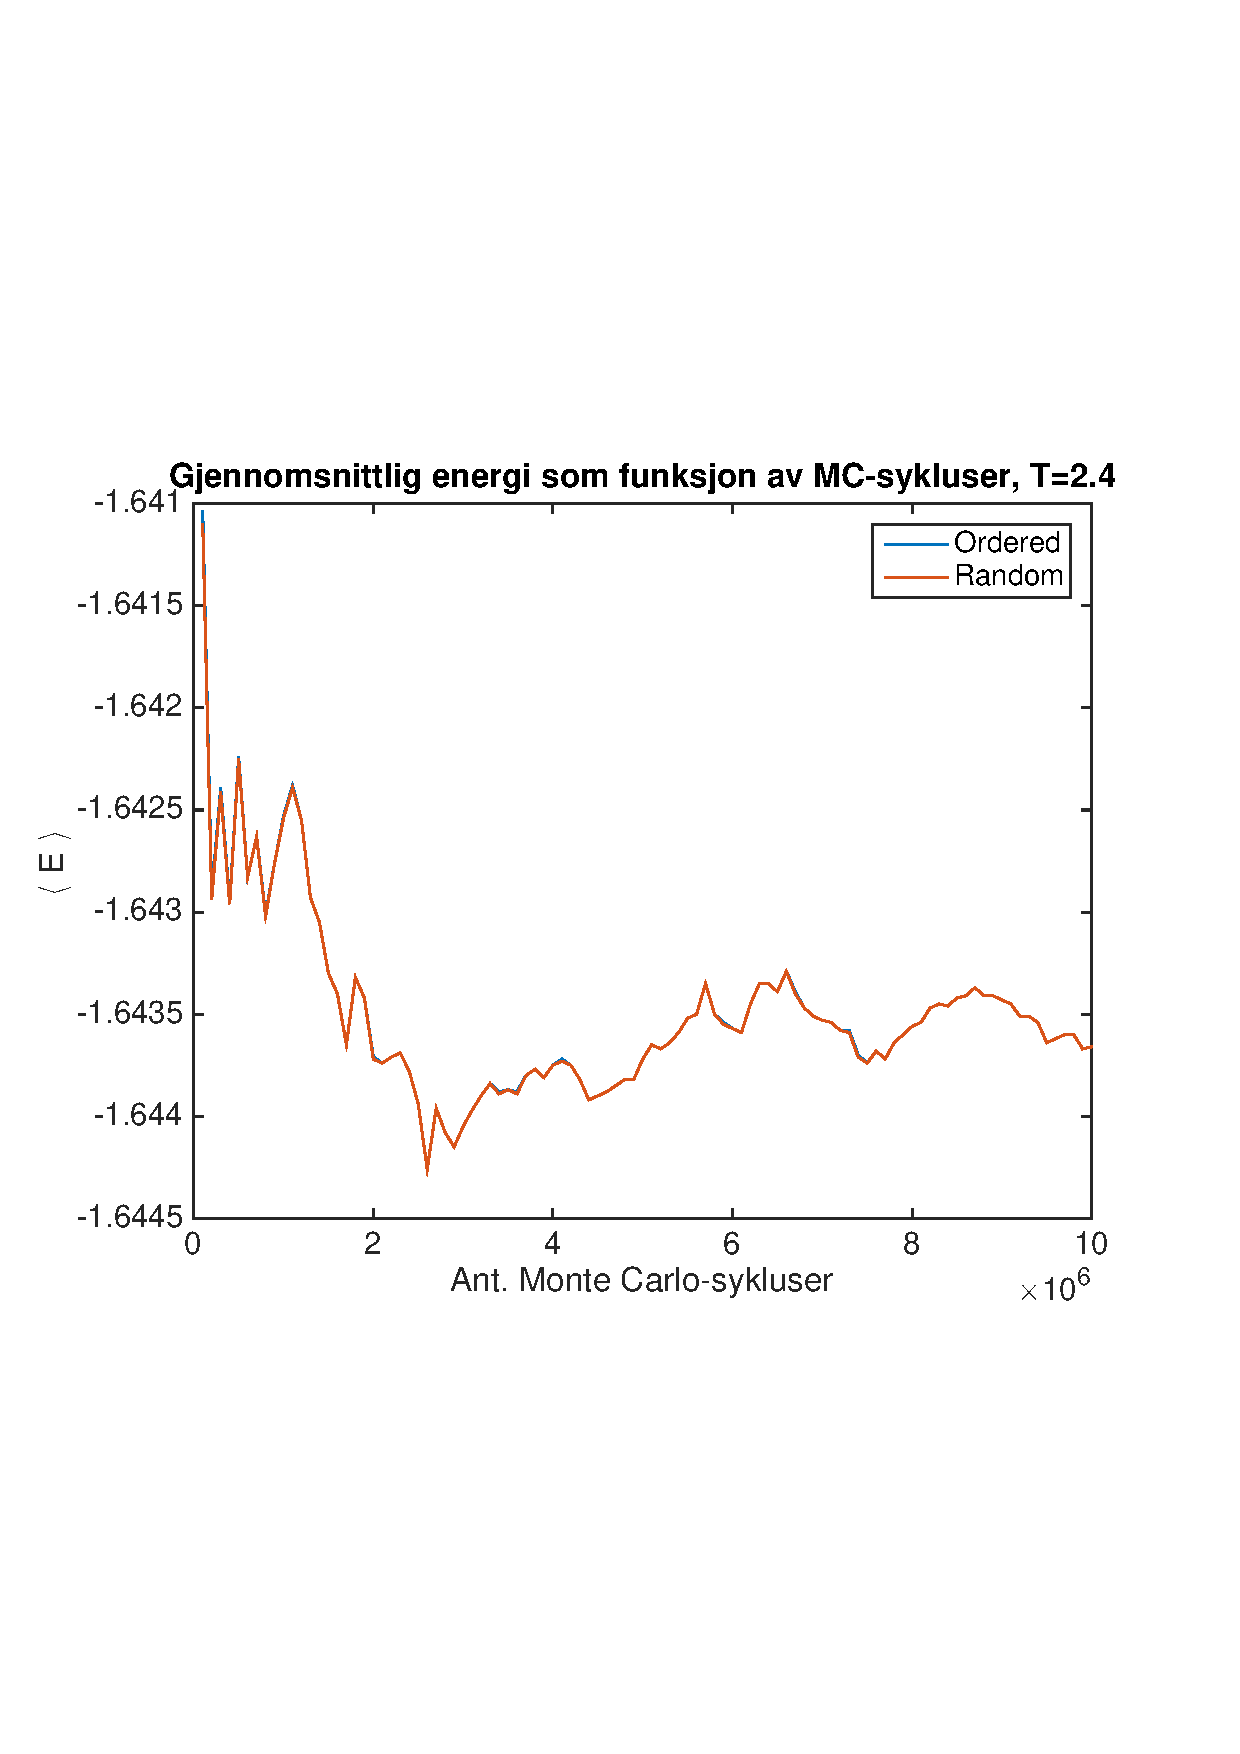
\includegraphics[scale = 0.6, trim = 1cm 8cm 1cm 8cm]{b_avgEnergy_MC_L2_T24.pdf}
\caption{Her er $\mean E$ plottet som funksjon av antall MC-sykluser for ordnet og uordnet starttilstand. Vi ser at første verdi for snittenergien er ganske bra, den treffer på andre desimal, og tar seg raskt inn til likevektstilstanden. Standardavviket til systemet som startet ordnet er $\mean E$ er $\sigma_{\mean E} = 4.5503\cdot10^{-4}$, som er ganske bra, vi kan da se bort fra termaliseringsprosessen når vi kjører med $4\cdot10^6$ MC-sykluser.}
\label{fig:meanET24}
\end{figure}

\begin{figure}[H]
\centering
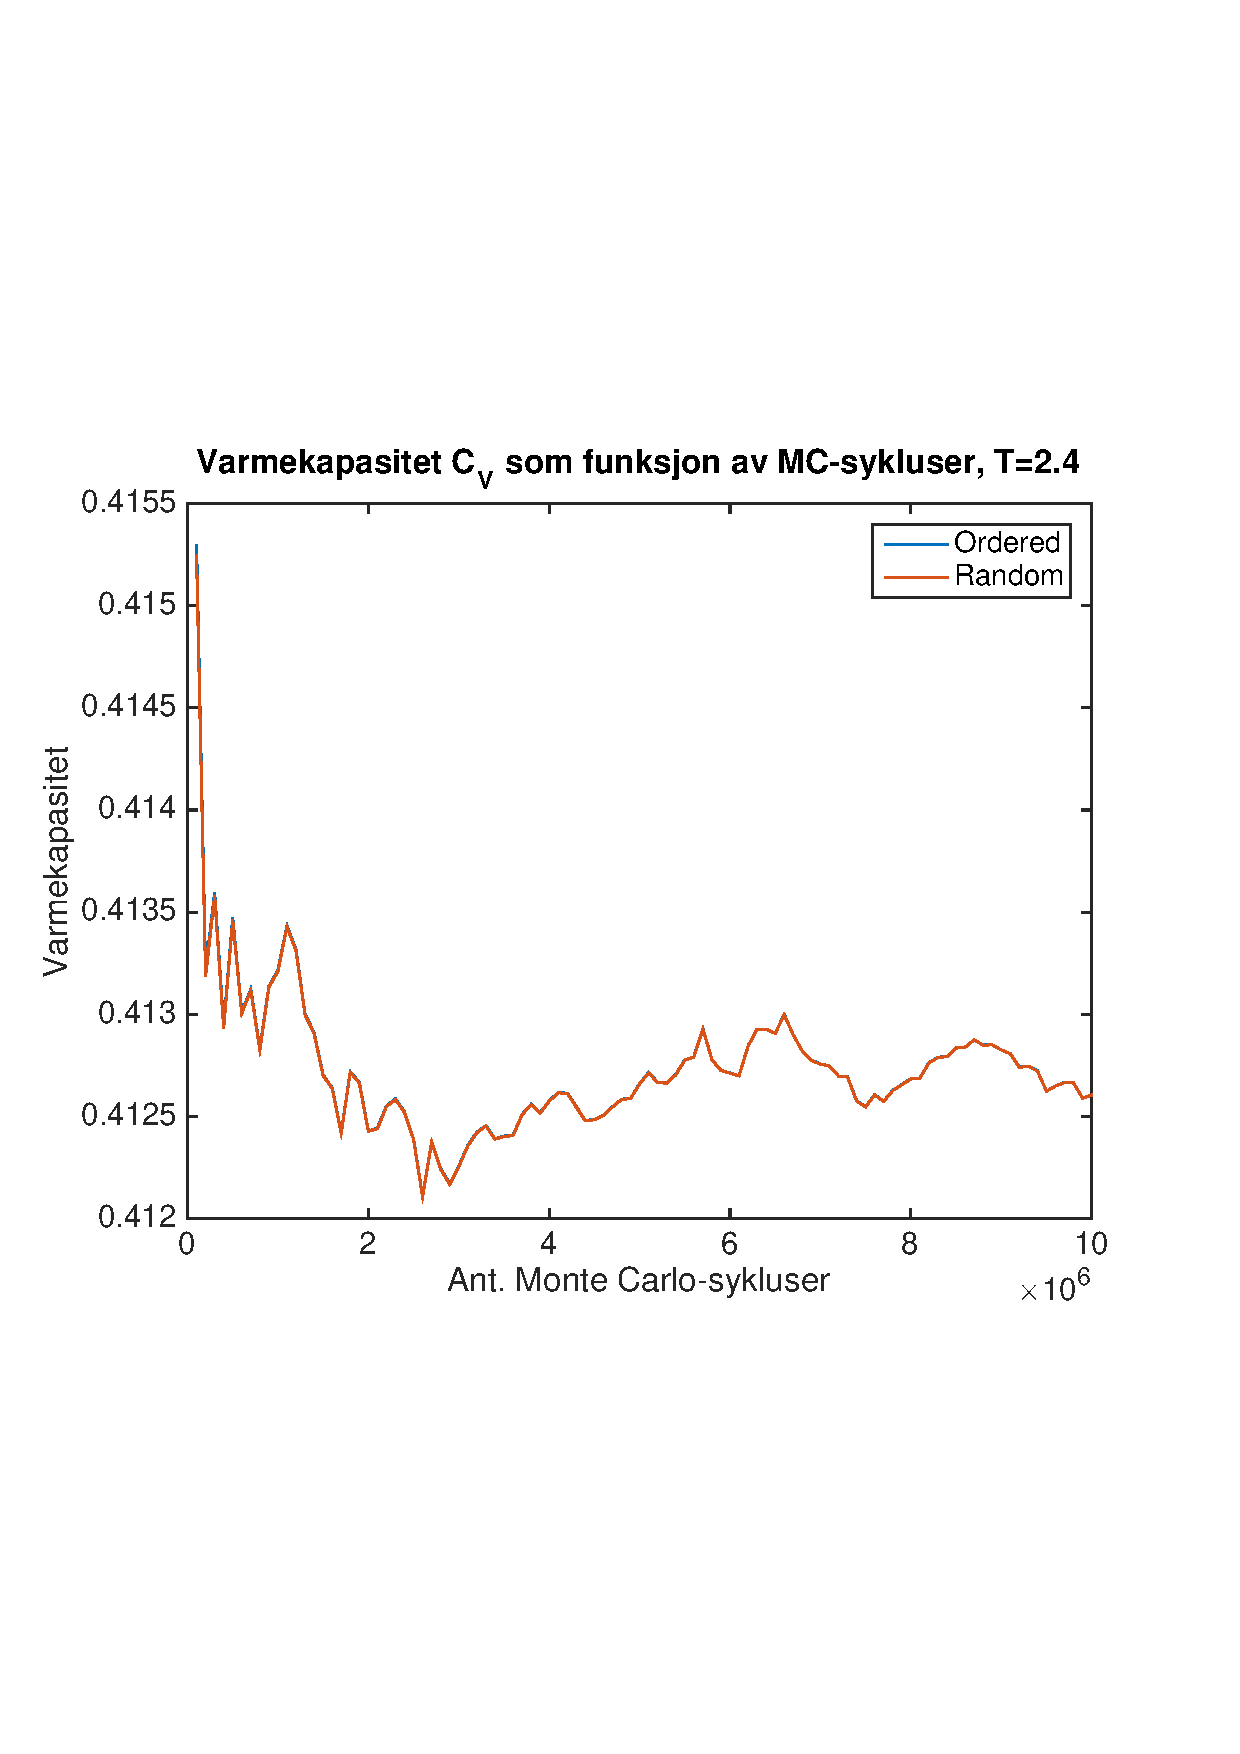
\includegraphics[scale = 0.6, trim = 1cm 8cm 1cm 8cm]{b_varmekap_MC_L2_T24.pdf}
\caption{Vi ser at varmekapasiteten blir estimert litt dårligere i starten enn snittenergien ble, men standardavviket er $\sigma_{C_V} = 3.6538\cdot10^{-4}$. Vi kan altså se bort fra termaliseringa her også.}
\label{fig:varmekapT24}
\end{figure}

\begin{figure}[H]
\centering
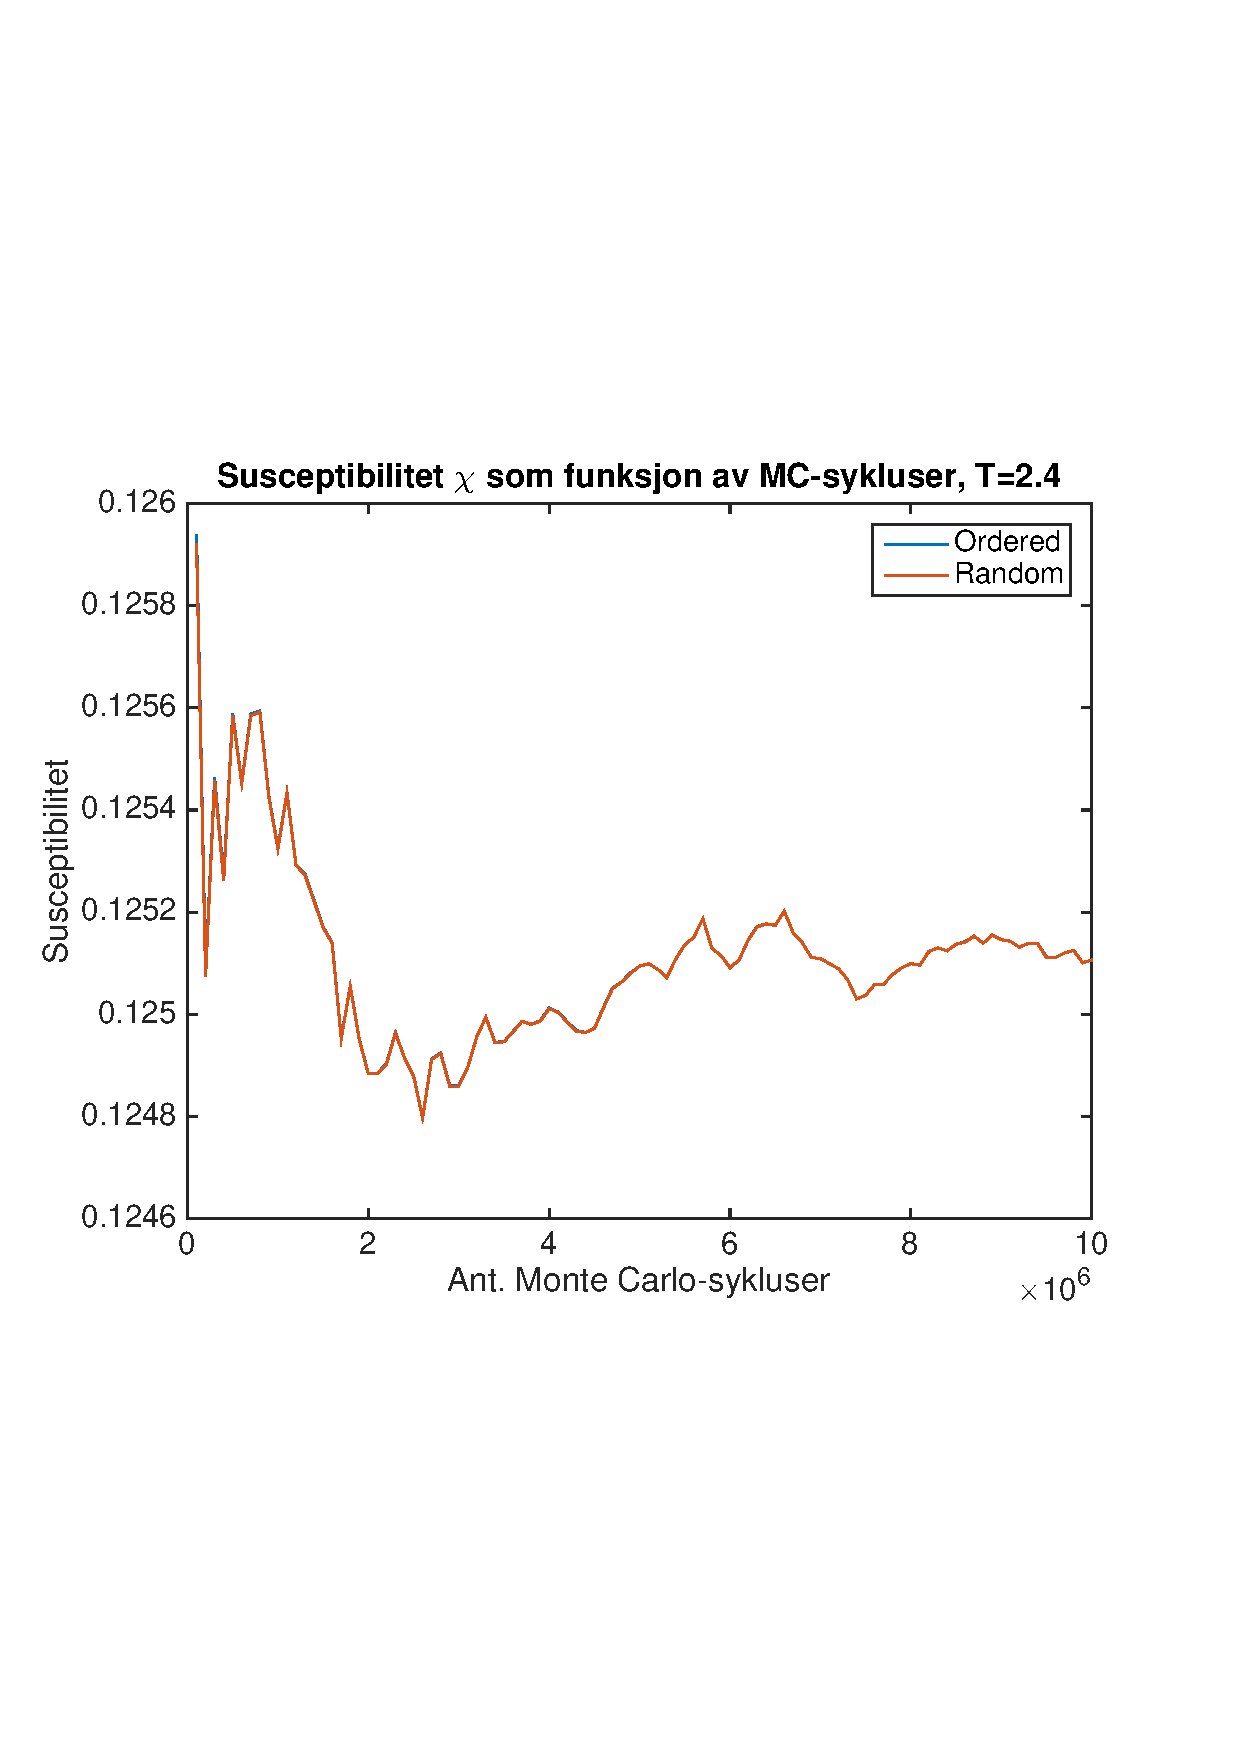
\includegraphics[scale = 0.6, trim = 1cm 8cm 1cm 8cm]{b_chi_MC_L2_T24.pdf}
\caption{Susceptibiliteten får et estimat som er et stykke unna likevektsverdien, men etter to millioner MC-sykluser er den så å si i likevekt. Standardavikket her er $\sigma_\chi = 1.7325\cdot10^{-5}$, som er det laveste av de tre verdiene vi har målt så langt.}
\label{fig:chiT24}
\end{figure}

\begin{figure}[H]
	\centering
	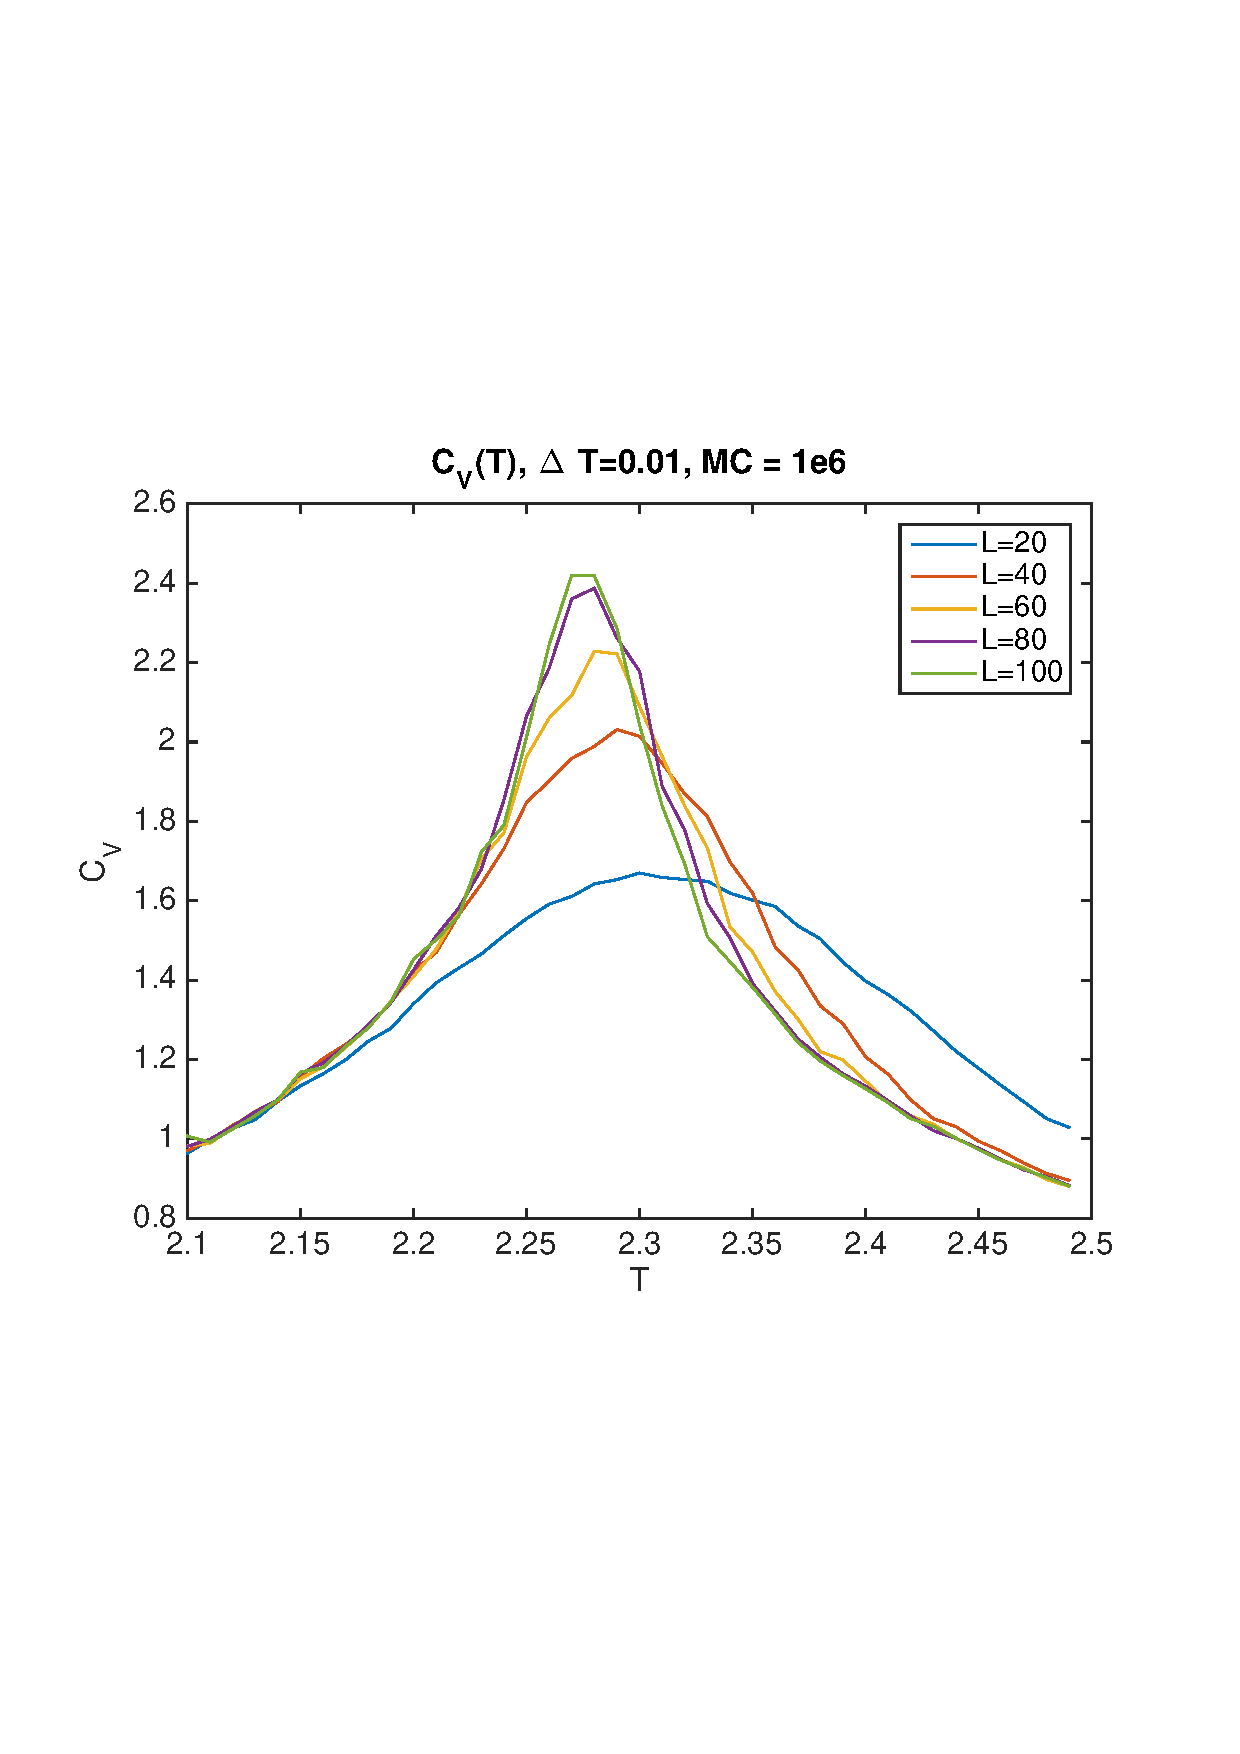
\includegraphics[scale = 0.6, trim = 1cm 8cm 1cm 8cm]{cv_difftemp.pdf}
	\caption{Varmekapasiteten ser ut til å konvergere mot en verdi etter som gitterstørrelsen øker, vi ser også en indikasjon på at noe skjer i området mellom $T=2.25$ og $T = 2.30$.}
	\label{fig:cv_difftemp}
\end{figure}

\begin{figure}[H]
	\centering
	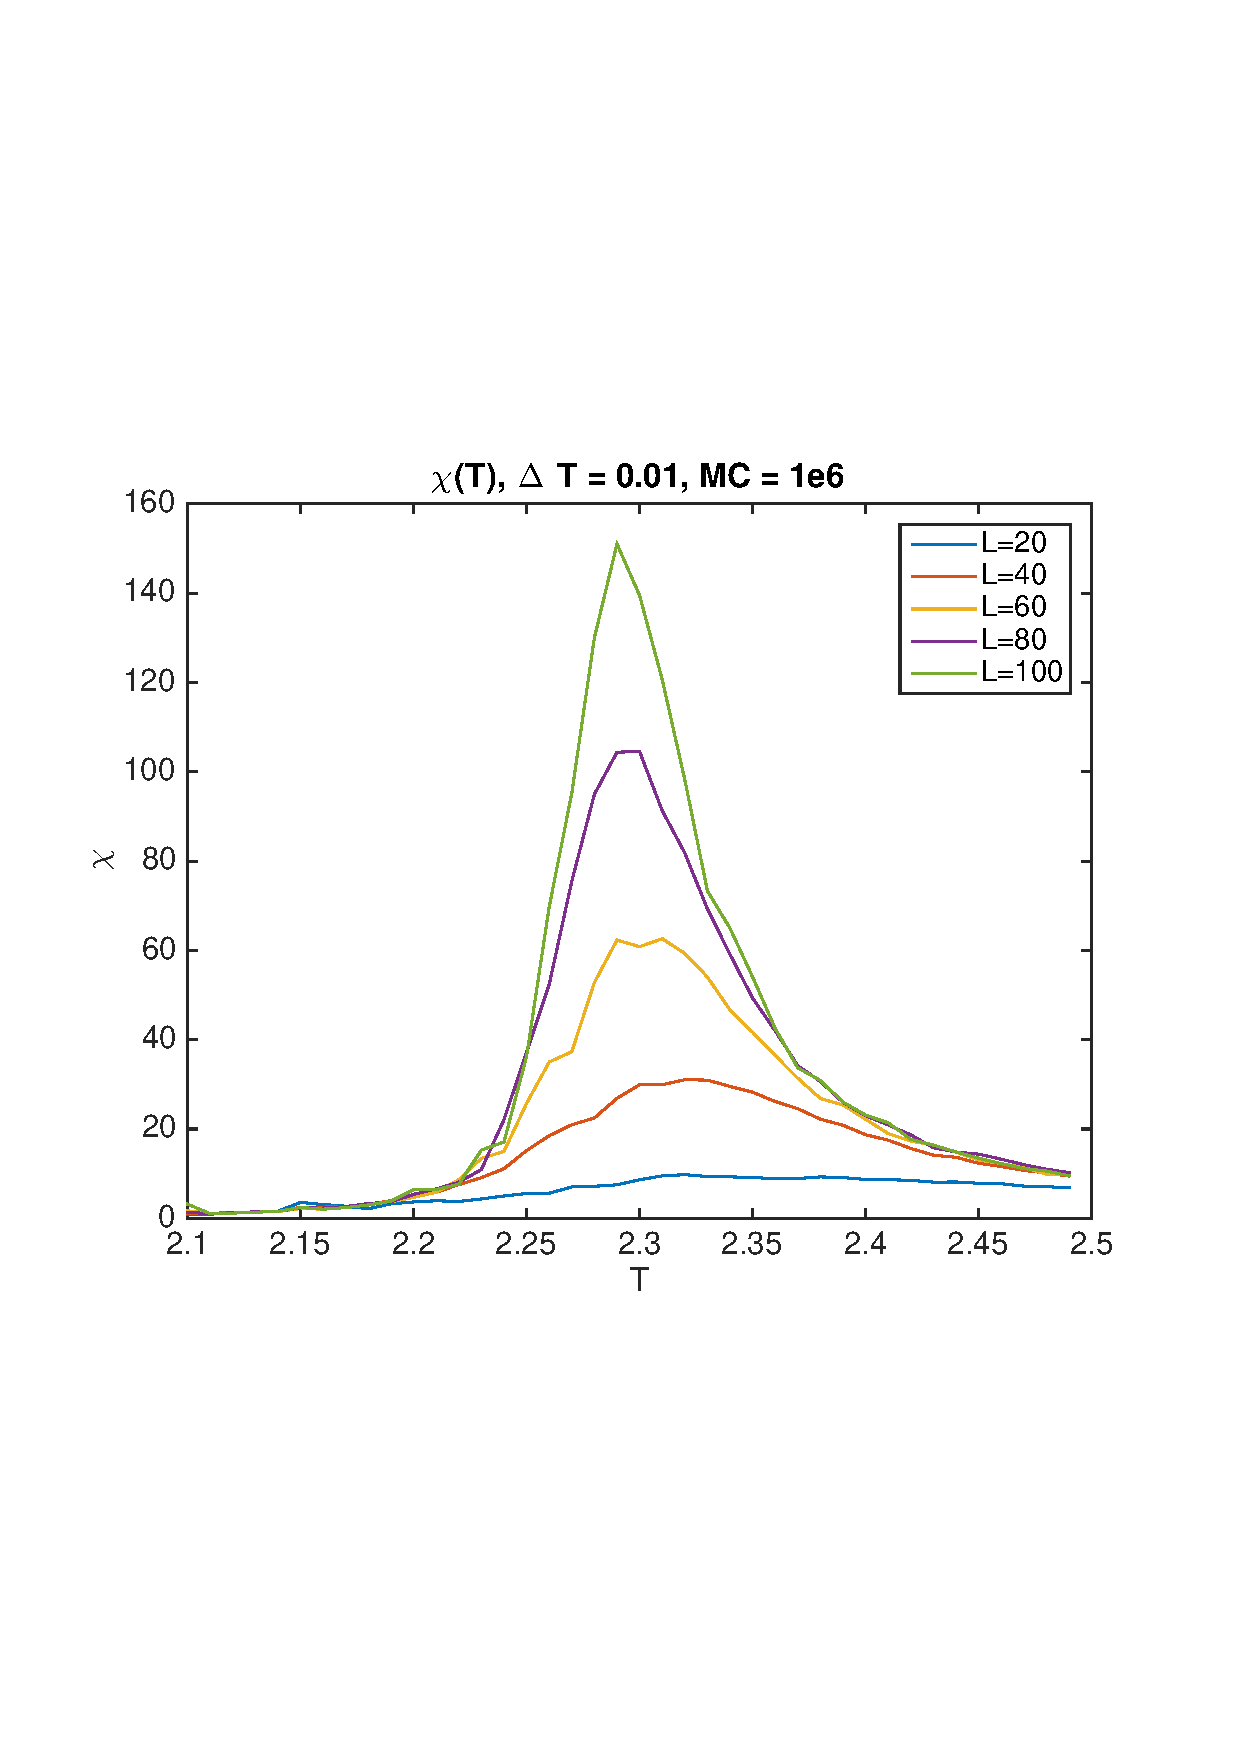
\includegraphics[scale = 0.6, trim = 1cm 8cm 1cm 8cm]{chi_difftemp.pdf}
	\caption{Her har vi plottet susceptibiliteten som funksjon av temperatur for flere gitterstørrelser. Vi ser klart at det skjer noe for $T\approx 2.3$. Dette noe er en faseovergang, i fig. (\ref{}) ser vi et estimat for faseovergangstemperaturen.}
	\label{fig:chi_difftemp}
\end{figure}

\begin{figure}[H]
	\centering
	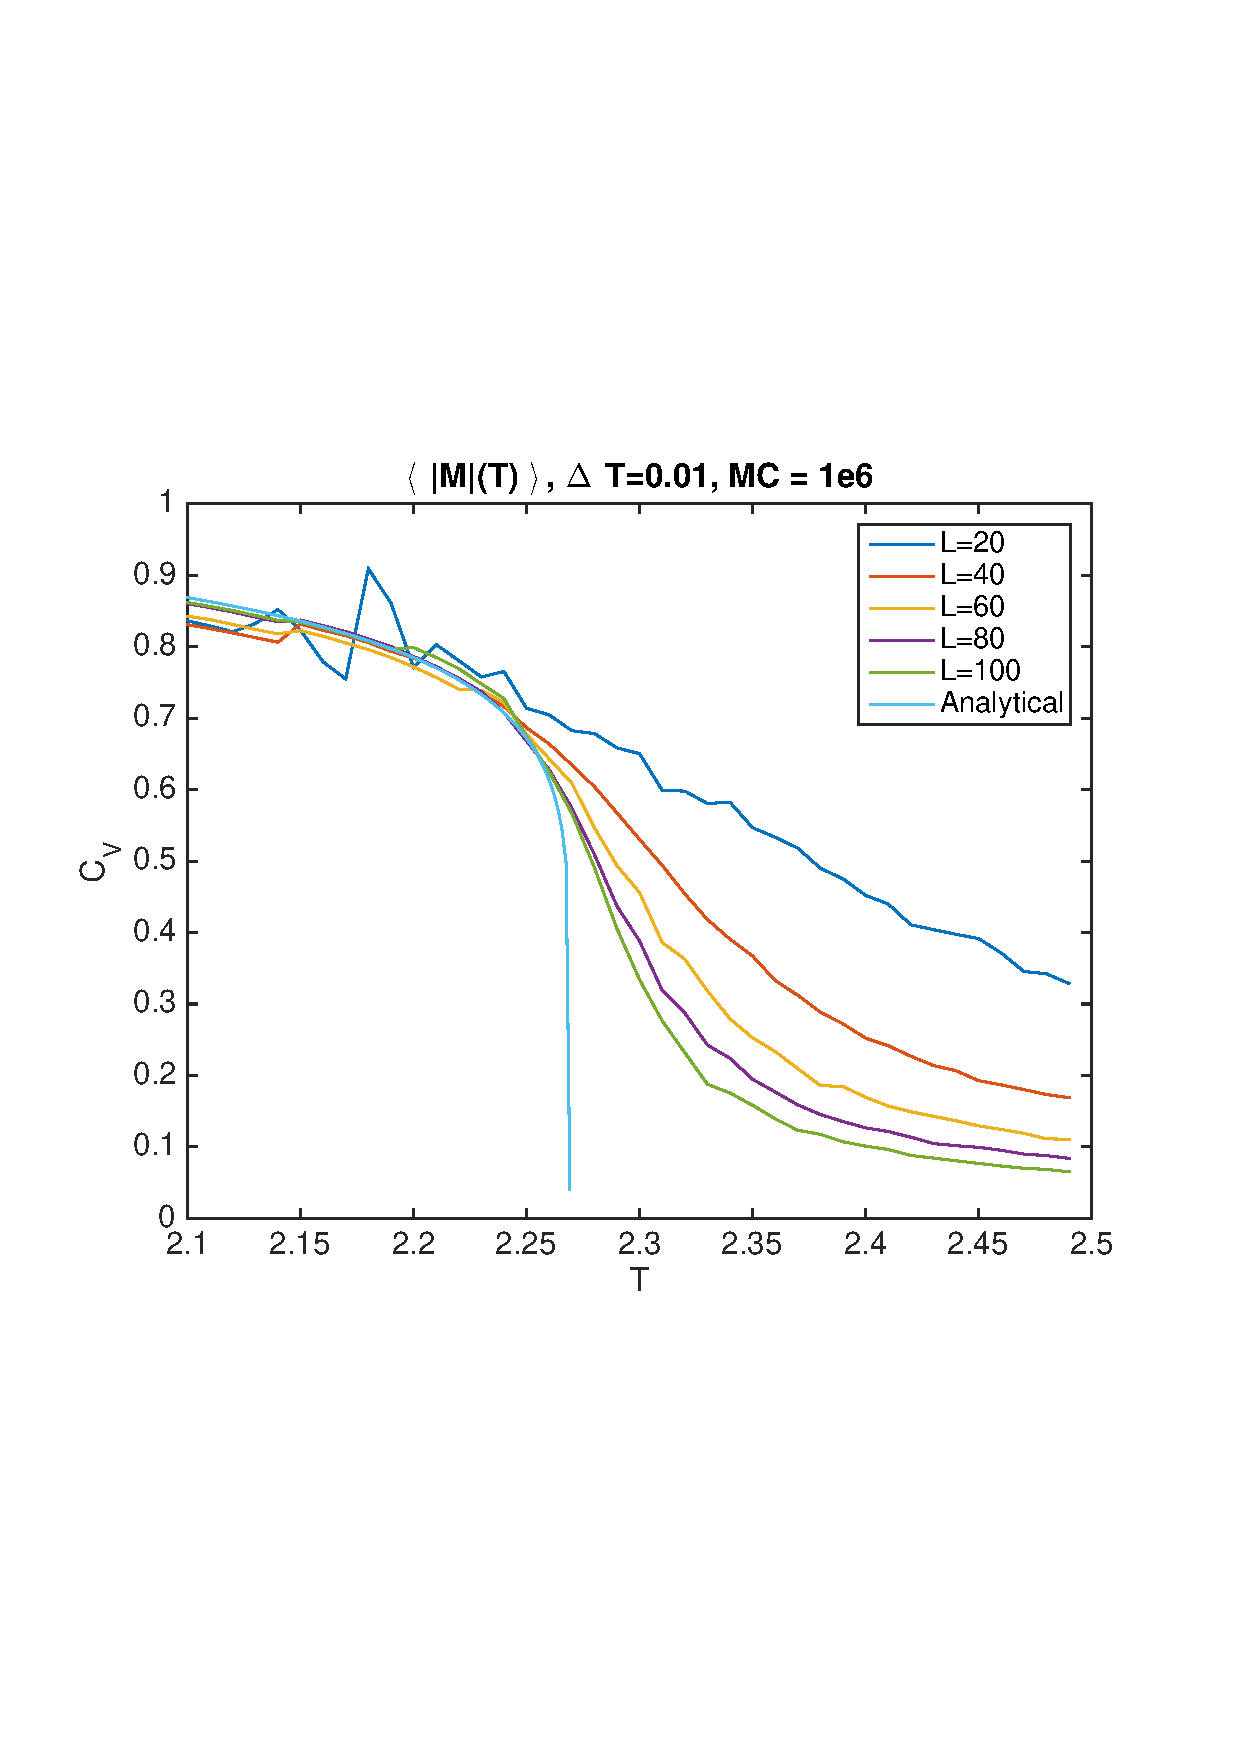
\includegraphics[scale = 0.6, trim = 1cm 8cm 1cm 8cm]{avg_mag_num_anal.pdf}
	\caption{Onsagers analytiske løsning er her plottet sammen med våre numeriske løsninger, vi ser at våre numeriske løsninger konvergerer fint mot den analytiske. Vi ser at over den kritiske temperaturen $T_C$ så har systemet null magnetisering.}
	\label{fig:avgmagnumanal}
\end{figure}

\begin{table}[H]
  \centering
  \begin{tabular}{ l l l l l}
    \toprule
    $I_{\text{Legendre}}$ & $I_{\text{Laguerre}}$ & $\epsilon_{\text{Legendre}}$ & $\epsilon_{\text{Laguerre}}$ & n \\
    \midrule
	0.129834 & 0.181567 & 0.326466 & 0.058093 & 10 \\
	0.199475 & 0.195887 & 0.034804 & 0.016192 & 15 \\
	0.177065 & 0.195636 & 0.081449 & 0.014892 & 20 \\
	0.189110 & 0.195240 & 0.018967 & 0.012837 & 25 \\
	0.185796 & 0.195070 & 0.036158 & 0.011955 & 30 \\
	\bottomrule
  \end{tabular}
  \caption{Resultat fra kjøringer av begge GK-metodene. Ingen av de er spesielt gode sammenliknet med Monte Carlo-metodene. Når vi hadde ti integrasjonspunkter så betydde det $10^6$ utregninger siden det var en seksdobbel løkke, en lite effektiv måte å angripe problemet på.}
  \label{tab:gauleg}
\end{table}

\section*{Numerisk stabilitet og presisjon}

\subsection*{Konklusjon}

\end{document}